\section{Software Explanation}

The final version here presented is a software that can be divided in the following parts: Hand Segmentation, Hand Description, Gesture Interface.

\subsection{Hand Segmentation}
The segmentation of the hand was one of the most important parts of the software since in it depends the correct functioning of the next parts. 
The flowchart of the segmentation of the code is as follows: 

\begin{center}
 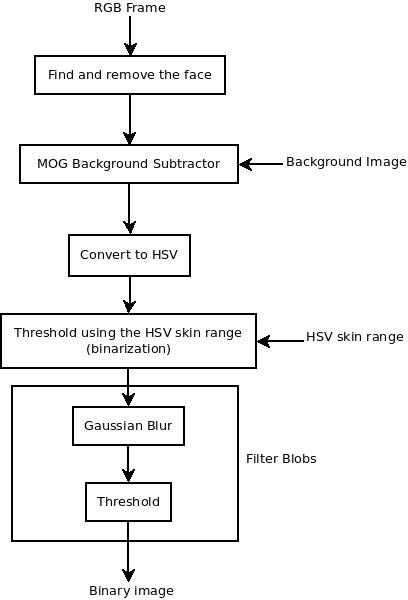
\includegraphics[scale=0.4]{../hand_filter.jpeg} 
 \end{center} 
 
As it can be seen in the diagram, the first thing done is to detect the face using the "Face Detection using Haar Cascades" already implemented in OpenCV. After this detection, a binary mask is made in which appear a black square over the face to hide it.

Next, a Mixture of Gaussians background subtractor is used to remove the background of the image and detect more easily the hand. From this step, another binary mask is created. 

Afterwards, the resulting image with the latter masks being applied is converted to the HSV color space and is thresholded using the appropriate HSV skin range.

Finally, in order to better the output binary image, a gaussian blur and a thresholding is applied to eliminate blobs and unite different regions of the hand. It was chosen this configuration because it was much faster and gave better results than making an opening to the image. 

 
\subsection{Hand Description}

The input of this section is the binary image that was the output of the previous one. This part of the software characterizes and extracts the hand's parameters. 
The flowchart is as follows: 

\begin{center}
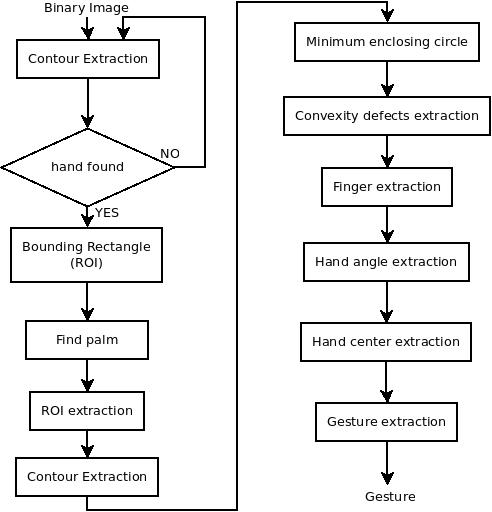
\includegraphics[scale=0.5]{../hand_description.jpeg} 
\end{center}

As it can be seen in the diagram, the first step is to extract the contours of the hand and decide from its size if it is a hand or only a blob remaining from the hand segmentation. 

If the size is appropriate, a bounding rectangle is found. Afterwards, the palm is extracted. In order to do that, a raw center of the palm and the radius of the inscribed circle is obtained from the points of the contour.

Then, the ROI (Region Of Interest), i.e. the rectangle that contains the maximum circle that represents the hand boundary.  

Afterwards, another contour extraction inside the extracted ROI is made in order to eliminate once more the smaller contours that may appear. 

Using the largest contour found in this last step, the minimum enclosing circle is obtained. This circle will be used as a hand's descriptor.

The following step is to compute the convexity defects, that will be used to extract the number of fingers present in the image. 
In order to assure that a certain part of the image is a finger, three conditions must be fulfilled: 
\begin{itemize}
\item The depth of the convexity defect must be in between the minimum inscribed radius and the maximum inscribed radius. 
\item The angle between the possible fingertips must be less than 90º. 
\item The fingertips must have a k-curvature inside a certain range.
\end{itemize}

In the next stage of the process, the angle of the hand is obtained measuring the angle of the minimum bounding box. A Kalman filter is placed in order to smooth the response of the system to sudden changes, that are assumed to be errors. 

Then, the hand center location is extracted using the center of the maximum inscribed circle and another Kalman filter to predict the position and eliminate the noise. 

Finally, the gesture made by the hand is extracted, taking as descriptors the number of fingers, the angle between fingers, and both the maximum and minimum inscribed circles. 

The output of this part of the software is a number that encodes the type of gesture made by the user.


\subsection{Gesture Interface} 
This section of the software has as an input the output of the previous, again. Hence, it will implement a state machine that, depending on the input (the gesture) will execute one function or other. 

\begin{center}
%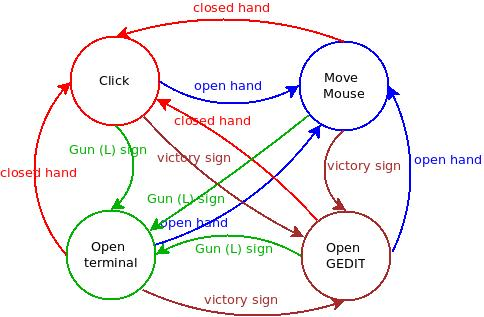
\includegraphics[scale=0.6]{../gesture_recognition.jpeg} 
\end{center}

The configuration of the actions to be made when an opened or closed palm appears is hardcoded in the program, since those values will not be changeables. In order to obtain the action for each of the two other gestures that may be customized, the software will read the configuration file, and execute the action specified in there. 

More information about the configuration file, the gestures and how to use the software in the following section "User Guide". 